%%%%%%%%%%%%%%%%%%%%%%%%%%%%%%%%%%%%%%%%%%%%%%%%%%%%%%%%%%%%%%%%%%%%%%%%%%
%                                                                        %
%  The Why platform for program certification                            %
%                                                                        %
%  Copyright (C) 2002-2014                                               %
%                                                                        %
%    Jean-Christophe FILLIATRE, CNRS & Univ. Paris-sud                   %
%    Claude MARCHE, INRIA & Univ. Paris-sud                              %
%    Yannick MOY, Univ. Paris-sud                                        %
%    Romain BARDOU, Univ. Paris-sud                                      %
%                                                                        %
%  Secondary contributors:                                               %
%                                                                        %
%    Thierry HUBERT, Univ. Paris-sud  (former Caduceus front-end)        %
%    Nicolas ROUSSET, Univ. Paris-sud (on Jessie & Krakatoa)             %
%    Ali AYAD, CNRS & CEA Saclay      (floating-point support)           %
%    Sylvie BOLDO, INRIA              (floating-point support)           %
%    Jean-Francois COUCHOT, INRIA     (sort encodings, hyps pruning)     %
%    Mehdi DOGGUY, Univ. Paris-sud    (Why GUI)                          %
%                                                                        %
%  This software is free software; you can redistribute it and/or        %
%  modify it under the terms of the GNU Lesser General Public            %
%  License version 2.1, with the special exception on linking            %
%  described in file LICENSE.                                            %
%                                                                        %
%  This software is distributed in the hope that it will be useful,      %
%  but WITHOUT ANY WARRANTY; without even the implied warranty of        %
%  MERCHANTABILITY or FITNESS FOR A PARTICULAR PURPOSE.                  %
%                                                                        %
%%%%%%%%%%%%%%%%%%%%%%%%%%%%%%%%%%%%%%%%%%%%%%%%%%%%%%%%%%%%%%%%%%%%%%%%%%

\documentclass[a4paper,11pt,twoside,openright]{report}
\usepackage{hevea}

\usepackage[pdftex,colorlinks=true,urlcolor=blue,pdfstartview=FitH]{hyperref}

\usepackage[latin1]{inputenc}
\usepackage[T1]{fontenc}
\usepackage{times}
\usepackage{amssymb}
%BEGIN LATEX
\usepackage{graphicx}
\newcommand{\negtenthspace}{\hspace*{-0.1\linewidth}}
%END LATEX
%HEVEA \newcommand{\includegraphics}[2][2]{\imgsrc{#2}}
%HEVEA \newcommand{\negtenthspace}{\relax}

\usepackage{color}
%\usepackage{mathptm}
%\usepackage{xspace}
\usepackage{makeidx}
\makeindex
\input{./version.tex}

% common Why title page

\newcommand{\whytitlepage}[4]{%
\begin{titlepage}
\begin{center}
~\vfill
\rule\textwidth{0.1cm}\\[0.5cm]
\begin{Huge}\sffamily
#1 % title
\end{Huge}
\\[1cm]
\begin{Large}\sffamily
#2
\end{Large}
\\[0.1cm]
\rule\textwidth{0.1cm}\\[1cm]
Version #3\\[3cm]
#4
\vfill
\today\\
INRIA Team-Project \emph{Proval} \url{http://proval.lri.fr} \\
INRIA Futurs \& LRI, CNRS UMR 8623\\ 
4, rue Jacques Monod, 91893 Orsay cedex, France
\end{center}
\end{titlepage}}

\newcommand{\why}{\textsf{Why}}
\newcommand{\Why}{\why}
\newcommand{\java}{\textsc{Java}\index{Java@\textsf{Java}}}
\newcommand{\Java}{\java}
\newcommand{\krakatoa}{\textsf{Krakatoa}\index{Krakatoa@\textsf{Krakatoa}}}
\newcommand{\Krakatoa}{\krakatoa}
\newcommand{\caduceus}{\textsf{Caduceus}\index{Caduceus@\textsf{Caduceus}}}
\newcommand{\Caduceus}{\caduceus}
\newcommand{\coq}{\textsf{Coq}\index{Coq@\textsf{Coq}}}
\newcommand{\Coq}{\coq}
\newcommand{\pvs}{\textsf{PVS}\index{PVS@\textsf{PVS}}}

%

\newcommand{\kw}[1]{\ensuremath{\mathsf{#1}}}

% types
\newcommand{\bool}{\kw{bool}}
\newcommand{\unit}{\kw{unit}}
%\newcommand{\tref}[1]{\ensuremath{#1~\kw{ref}}}
\newcommand{\tref}[1]{\ensuremath{#1~\mathsf{ref}}}
\newcommand{\tarray}[2]{\ensuremath{\kw{array}~#1~\kw{of}~#2}}

% constructs
\newcommand{\prepost}[3]{\ensuremath{\{#1\}\,#2\,\{#3\}}}
\newcommand{\result}{\ensuremath{\mathit{result}}}

\newcommand{\void}{\kw{void}}
\newcommand{\access}[1]{\ensuremath{!#1}}
\newcommand{\assign}[2]{\ensuremath{#1~:=~#2}}
\newcommand{\pref}[1]{\ensuremath{\kw{ref}~#1}}
\newcommand{\taccess}[2]{\ensuremath{#1\texttt{[}#2\texttt{]}}}
\newcommand{\tassign}[3]{\ensuremath{#1\texttt{[}#2\texttt{]}~\texttt{:=}~#3}}
\newcommand{\faccess}[2]{\ensuremath{(\mathit{access}~#1~#2)}}
\newcommand{\fupdate}[3]{\ensuremath{(\mathit{update}~#1~#2~#3)}}
%\newcommand{\taccess}[2]{\ensuremath{#1[#2]}}
%\newcommand{\tassign}[3]{\ensuremath{#1[#2]~:=~#3}}
%\newcommand{\faccess}[2]{\ensuremath{(\mathit{access}~#1~#2)}}
%\newcommand{\fupdate}[3]{\ensuremath{(\mathit{update}~#1~#2~#3)}}
% \newcommand{\block}[1]{\ensuremath{\kw{begin}~#1~\kw{end}}}
\newcommand{\seq}[2]{\ensuremath{#1;~#2}}
%\newcommand{\plabel}[2]{\ensuremath{#1:#2}}
\newcommand{\plabel}[2]{\ensuremath{#1\texttt{:}#2}}
\newcommand{\assert}[2]{\ensuremath{\kw{assert}~\{#1\};~#2}}
\newcommand{\while}[4]{\ensuremath{\kw{while}~#1~\kw{do}~\{\kw{invariant}~#2~\kw{variant}~#3\}~#4~\kw{done}}}
\newcommand{\ite}[3]{\ensuremath{\kw{if}~#1~\kw{then}~#2~\kw{else}~#3}}
\newcommand{\fun}[3]{\ensuremath{\kw{fun}~#1:#2\rightarrow#3}}
\newcommand{\app}[2]{\ensuremath{(#1~#2)}}
\newcommand{\rec}[4]{\ensuremath{\kw{rec}~#1:#2~\{\kw{variant}~#3\}=#4}}
\newcommand{\letin}[3]{\ensuremath{\kw{let}~#1=#2~\kw{in}~#3}}
\newcommand{\raisex}[2]{\ensuremath{\kw{raise}~(#1~#2)}}
\newcommand{\exn}[1]{\ensuremath{\kw{Exn}~#1}}
\newcommand{\try}[2]{\ensuremath{\kw{try}~#1~\kw{with}~#2~\kw{end}}}
\newcommand{\coerce}[2]{\ensuremath{(#1:#2)}}

\newcommand{\statement}{\textit{statement}}
\newcommand{\program}{\textit{program}}
\newcommand{\expression}{\textit{expression}}
\newcommand{\predicate}{\textit{predicate}}

% inference rules
\newcommand{\espacev}{\rule{0in}{1em}}
\newcommand{\espacevn}{\rule[-0.4em]{0in}{1em}}
\newcommand{\irule}[2]
  {\frac{\espacevn\displaystyle#1}{\espacev\displaystyle#2}}
\newcommand{\typage}[3]{#1 \, \vdash \, #2 : #3}
\newcommand{\iname}[1]{\textsf{#1}}

\newcommand{\emptyef}{\bot}
\newcommand{\wf}[1]{#1~\kw{wf}}
\newcommand{\pur}[1]{#1~\kw{pure}}
\newcommand{\variant}[1]{#1~\kw{variant}}

\newcommand{\wpre}[2]{\ensuremath{\mathit{wp}(#1,#2)}}
\newcommand{\wprx}[3]{\ensuremath{\mathit{wp}(#1,#2,#3)}}

\newcommand{\barre}[1]{\ensuremath{\overline{#1}}}

%%% Local Variables: 
%%% mode: latex
%%% TeX-master: "doc"
%%% End: 

\definecolor{darkgreen}{rgb}{0, 0.5, 0}

\setlength{\textheight}{240mm}
\setlength{\topmargin}{-10mm}
\setlength{\textwidth}{160mm}
\setlength{\oddsidemargin}{0mm}
\setlength{\evensidemargin}{0mm}

\renewcommand{\textfraction}{0.01}
\renewcommand{\topfraction}{0.99}
\renewcommand{\bottomfraction}{0.99}

\usepackage{fancyhdr}
\pagestyle{fancyplain}
\renewcommand{\footrulewidth}{0.4pt}
\addtolength{\headheight}{2pt}
\addtolength{\headwidth}{1cm}
\renewcommand{\chaptermark}[1]{\markboth{#1}{}}
\renewcommand{\sectionmark}[1]{\markright{\thesection\ #1}}
\lhead[\fancyplain{}{\bfseries\thepage}]{\fancyplain{}{\bfseries\rightmark}}
\chead{}
\rhead[\fancyplain{}{\bfseries\leftmark}]{\fancyplain{}{\bfseries\thepage}}
\lfoot{\fancyplain{}{C. March\'e, Y. Moy}}
\cfoot{\fancyplain{}{Why platform, Jessie plugin for Frama-C}}
\rfoot{\fancyplain{}{ProVal, \today}}


\begin{document}
%HEVEA This document is also available in \ahref{jessie.pdf}{PDF format}.
%BEGIN LATEX
\sloppy
\hbadness=9999
%END LATEX

\whytitlepage{The Jessie plugin\\~\\ for Deductive Verification in Frama-C}{Tutorial and Reference Manual}{\whyversion}{Claude March\'e, Yannick Moy}

\tableofcontents

\chapter{Introduction}

Jessie is a plugin for the Frama-C environment, aimed at performing
deductive verification of C programs, annotated using the ACSL
language~\cite{baudin09acsl}, using the \Why{}~\cite{why} tool for
generating proof obligations.

This version \whyversion{} of Jessie is compatible with Frama-C version
Nitrogen (and no other).

\section{Important note for version 2.30}

The use of the Why2 VC generator is now obsolete, and it is
recommended to switch to the Why3 system for specification and VC
generation. Why3 must be installed independently of Why2, please see the
instructions given at \url{http://why3.lri.fr}.

The version of Why3 that is compatible with this version \whyversion{} of Jessie
is the version 0.71. Please see \url{http://krakatoa.lri.fr/} for more
details on compatibility between Frama-C, Why2/Jessie and Why3.

In this manual, it is assumed that the Why3 VC generator and IDE is in
use.  The old behavior using the Why2 VC generator and GUI remains
possible, using option \texttt{-jessie-atp=gui}.

\section{Basic Use}

\begin{figure}[t]
  \begin{center}
    %HEVEA 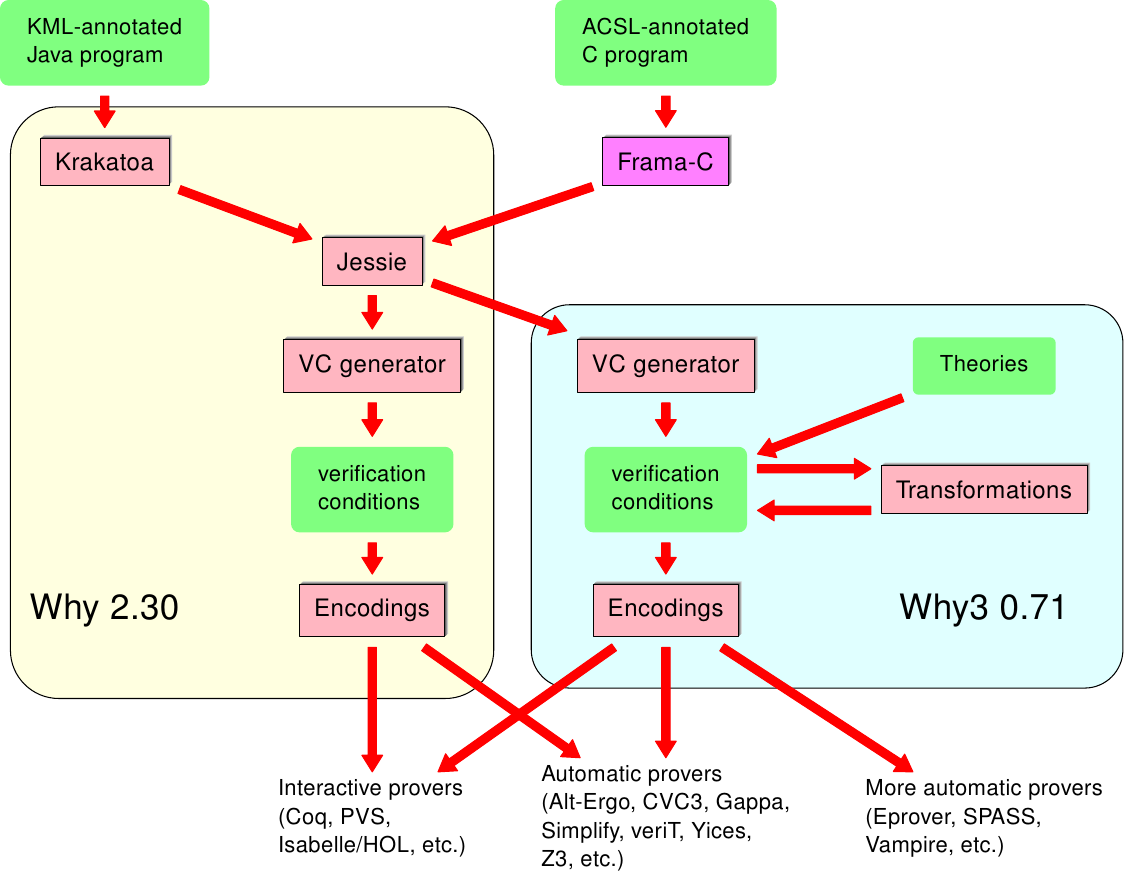
\includegraphics[width=0.8\linewidth]{why_frama_c2-mps.png}
    %BEGIN LATEX
    \includegraphics[width=0.8\linewidth]{why_frama_c2.mps}
    %END LATEX
  \end{center}
  \caption{Frama-C, the Why Platform and the new Why3 system}
  \label{fig:platform}
\hrulefill
\end{figure}

The Jessie plug-in allows to perform deductive verification of C
programs inside Frama-C. The C file possibly annotated in ACSL is
first checked for syntax errors by Frama-C core, before it is
translated to various intermediate languages inside the Why Platform
embedded in Frama-C, and finally verification conditions (VCs) are
generated and a prover is called on these, as sketched in
Figure~\ref{fig:platform}.

To prove the VCs generated, one needs to install external provers such
as Alt-Ergo, CVC3 or Z3. Please see at URL
\url{http://krakatoa.lri.fr/} how to get such provers. Once some of
these are installed, you should run the auto-configuration tool by
running command \texttt{why3config --detect} (equivalent to the
former Why 2.xx  command \texttt{why-config})

By default, the Jessie plug-in launches in its GUI mode. To invoke this
mode on a file \verb|ex.c|, just type

\begin{verbatim}
> frama-c -jessie ex.c
\end{verbatim}

A program does not need to be complete to be analyzed with the Jessie
plug-in. As a first example, take program \verb|max|:
\input{texpp/max.cpp} The ACSL annotation expresses the fact function
\verb|max| returns the maximum of its parameters \verb|i| and
\verb|j|. Now, running the Jessie plug-in launches Why3 IDE produces
the output shown on Figure~\ref{fig:max:ide}.

\begin{figure}[t]
  \begin{center}
    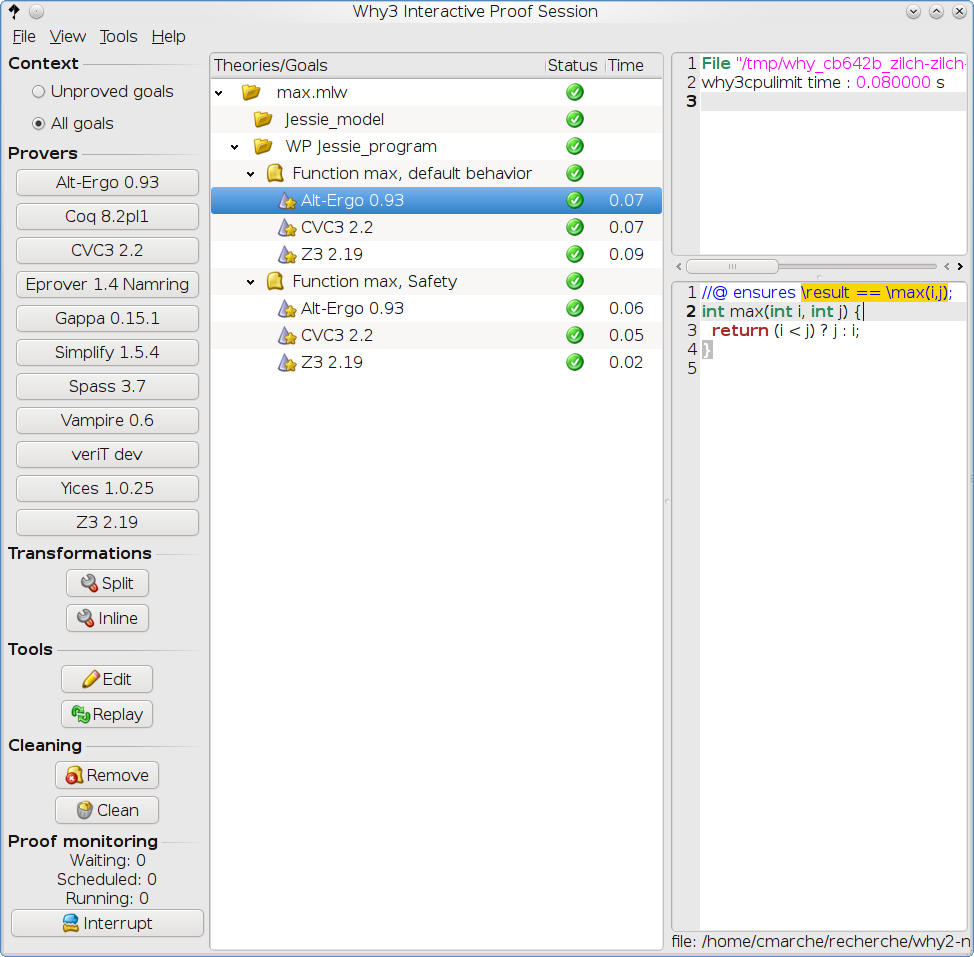
\includegraphics[width=\linewidth]{jessie/max_why3ide.png}
  \end{center}
  \caption{Why3 IDE for \texttt{max} function}
  \label{fig:max:ide}
\end{figure}

On this figure, the user selected the row ``WP Jessie program'' and
clicked on the buttons on the left, corresponding to provers Alt-Ergo,
Z3 and CVC3. The two VCs are shown valid, meaning that for this small
function, the code matches its specification.

\section{Safety Checking vs. Functional Verification}

In the simple \verb|max| example, there are two VCs, one for the
``default behavior'' and one for ``Safety'' of function \verb|max|. In
general, each function leads to these VCs:
\begin{itemize}
\item \textit{Safety}: this VC guard against safety violations
  such as null-pointer dereferencing, buffer overflow, integer overflow, etc.
\item \textit{Default behavior}: this VC concern the
  verification of a function's default behavior, which includes
  verification of its postcondition, frame condition, loop invariants
  and intermediate assertions.
\item \textit{User-defined behavior}: these VCs concern the
  verification of a function's user-defined behavior, which includes
  verification of its postcondition, frame condition, loop invariants
  and intermediate assertions for this specific behavior.
\end{itemize}

Here is a more complex variant of function \verb|max| which takes
pointer parameters and returns 0 on success and -1 on failure.

\input{texpp/max_ptr.cpp}

Notice that the annotations refer to the null pointer using ACSL
syntax \verb|\null|. It would be possible to use also the C macro
\texttt{NULL}, but in that case we would have to ask Frama-C
preprocessor phase to process the annotations too, since it does not
by default. This is done by option \verb|-pp-annot| of
Frama-C. However, this alternative is not recommended since it 
depends of the proprecessor in use (see
\url{http://bts.frama-c.com/dokuwiki/doku.php?id=mantis:frama-c:start#faq_tips_and_tricks})

Running the Jessie plug-in in GUI mode results in 4 VCs:
Safety, default behavior, normal behavior `normal` and normal behavior
`zero` for the two user-defined behaviors.

\begin{figure}[t]
  \begin{center}
    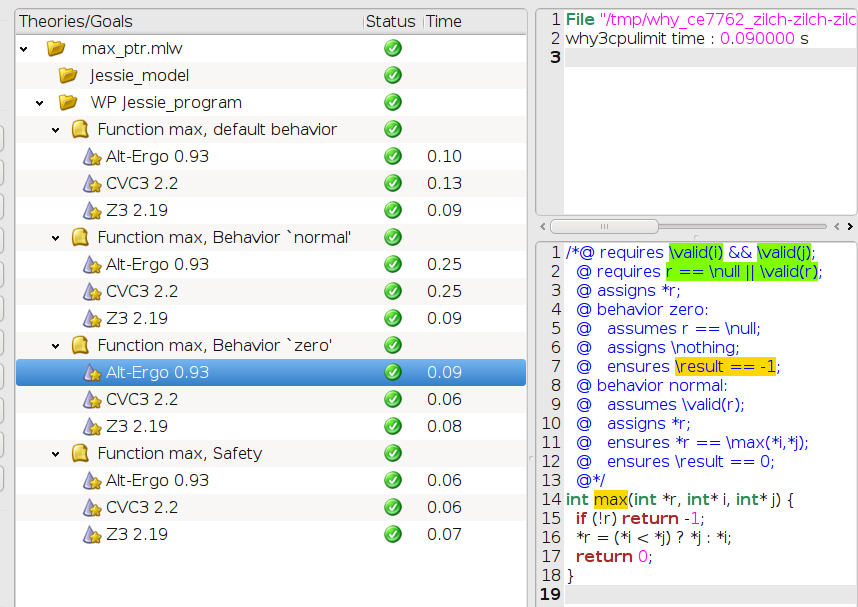
\includegraphics[width=\linewidth]{jessie/max_ptr_why3ide.png}
  \end{center}
  \caption{Why3 IDE for \texttt{max\_ptr} function}
  \label{fig:max_ptr:ide}
\end{figure}

% VCs that are proved in one group can be available to prove VCs in other
% groups. No circularity paradox is possible here, since the proof of a
% VC can only rely on other VCs higher in the control-flow graph of the
% function. We made the following choices:

% \begin{itemize}
% \item To prove a VC in \textit{Safety}, one can rely on VCs in
%   \textit{Default behavior}. Typically, one can rely on preconditions
%   or loop invariants to prove safety.
% \item To prove a VC in \textit{Default behavior}, one can rely on VCs
%   in \textit{Safety}. Typically, one can rely on ranges of values
%   implied by safety to prove loop invariants and postconditions.
% \item To prove a VC in a \textit{Normal behavior}, one can rely on VCs
%   in both \textit{Safety} and \textit{Default behavior}.
% \end{itemize}

In the next chapters, we detail how to prove each kind of VC.
We also recommend to
look at the collection of verified programs at URL
\url{http://proval.lri.fr/gallery/jessieplugin.en.html} to get more hints
on how to specify and prove programs with Jessie.

\chapter{Safety Checking}

A preliminary to the verification of functional properties using the
Jessie plug-in is to verify the safety of functions. Safety has
several components: memory safety, integer safety, termination. Memory
safety deals with validity of memory accesses to allocated
memory. Integer safety deals with absence of integer overflows and
validity of operations on integers, such as the absence of division by
zero. Termination amounts to check whether loops are always
terminating, as well as recursive or mutually recursive functions.

\section{Memory Safety}

Our running example will be the famous \verb|binary_search| function,
which searches for a {\tt long} in an ordered array of {\tt long}s. On
success, it returns the index at which the element appears in the
array. On failure, it returns \verb|-1|.

\input{texpp/binary_search_raw.cpp}

To concentrate first on memory safety only, we declare two pragmas as
above. The first pragma dictates that integers in C programs behave as
infinite-precision mathematical integers, without overflows. The
second pragma instructs the plug-in to ignore termination issues.

Let's call Frama-C with the Jessie plug-in on this program:

\begin{verbatim}
> frama-c -jessie binary-search.c
\end{verbatim}

Figure~\ref{fig:raw} shows the result after
\begin{itemize}
\item clicking on Alt-Ergo button to launch Alt-Ergo on both Safety
  and Normal behavior. The normal behavior is proved valid but not the safety.
\item selecting the raw ``safety'' and clicking on the button
  ``split'' to split the VC in parts. 3 sub-goals are obtained: one that states the divisor \verb|2| is not null, and two more that state the
array access \verb|t[m]| should be within bounds. 
\item clicking again on Alt-Ergo, then CVC3 then Z3
\end{itemize}

\begin{figure}[t]
  \begin{center}
  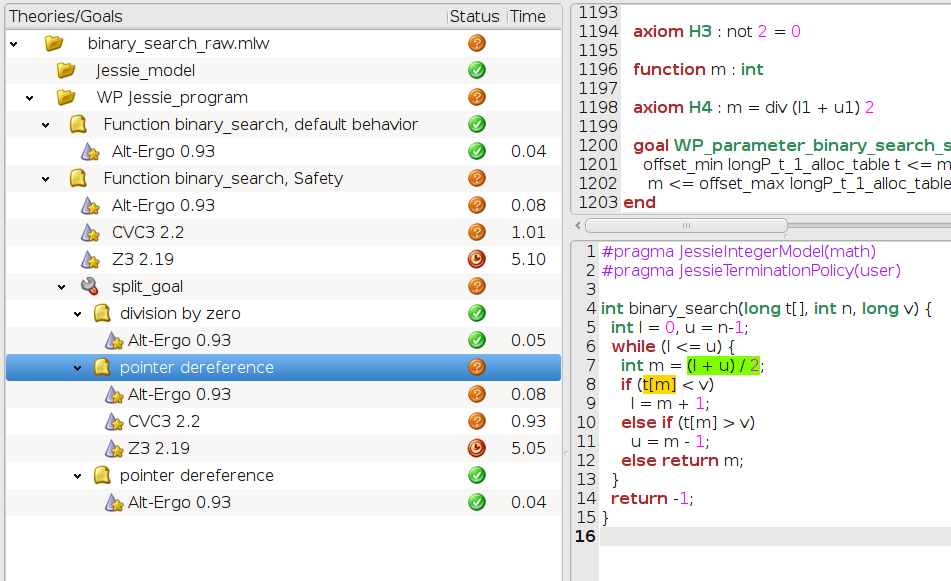
\includegraphics[width=1.0\linewidth]{jessie/binary_search_raw.png}
  \end{center}
  \caption{Memory safety with no annotations}
  \label{fig:raw}
  \hrulefill
\end{figure}

The remaing VC cannot be proved. Indeed, it is false that, in any
context, function \verb|binary_search| is memory safe. To ensure
memory safety, \verb|binary_search| must be called in a context where
\verb|n| is positive and array \verb|t| is valid between indices
\verb|0| and \verb|n-1| included. Since function \verb|binary_search|
accesses array \verb|t| inside a loop, providing a precondition is not
enough to make the generated VC provable.  One must also provide a
\emph{loop invariant}. A loop invariant is a property that remains
true at each iteration of the loop.  It is often necessary for the
user to provide these properties to help Jessie reason about
loops. Assuming that the right property has been provided, Jessie is
then left with the easier task of generating and verifying VCs that
ensure that the property indeed holds at the beginning of each
iteration.

In this example, it is necessary to provide an invariant that states
the guarantees provided on the array index, despite its changing
value. It states that the value of index \verb|l| stays within the
bounds of the array \verb|t|.

\input{texpp/binary_search_rawmem.cpp}

Launching again the IDE after adding these annotations, you should
obtain that all VCs are now proved.

\section{Integer Overflow Safety}

Let us now consider machine integers instead of idealized mathematical
integers. This is obtained by removing the pragma
\texttt{JessieIntegerModel}.  Without this pragma, integer types are
now interpreted as bounded machine integers. However, the default is a
\emph{defensive} interpretation, which forbids the arithmetic
operations to overflow.\footnote{In a context where it is intended for
  the operations to overflows, and thus operations are intentionnally
  done modulo, the same pragma should be set to the value
  \texttt{modulo}, see Jessie manual.}

\begin{figure}[t]
  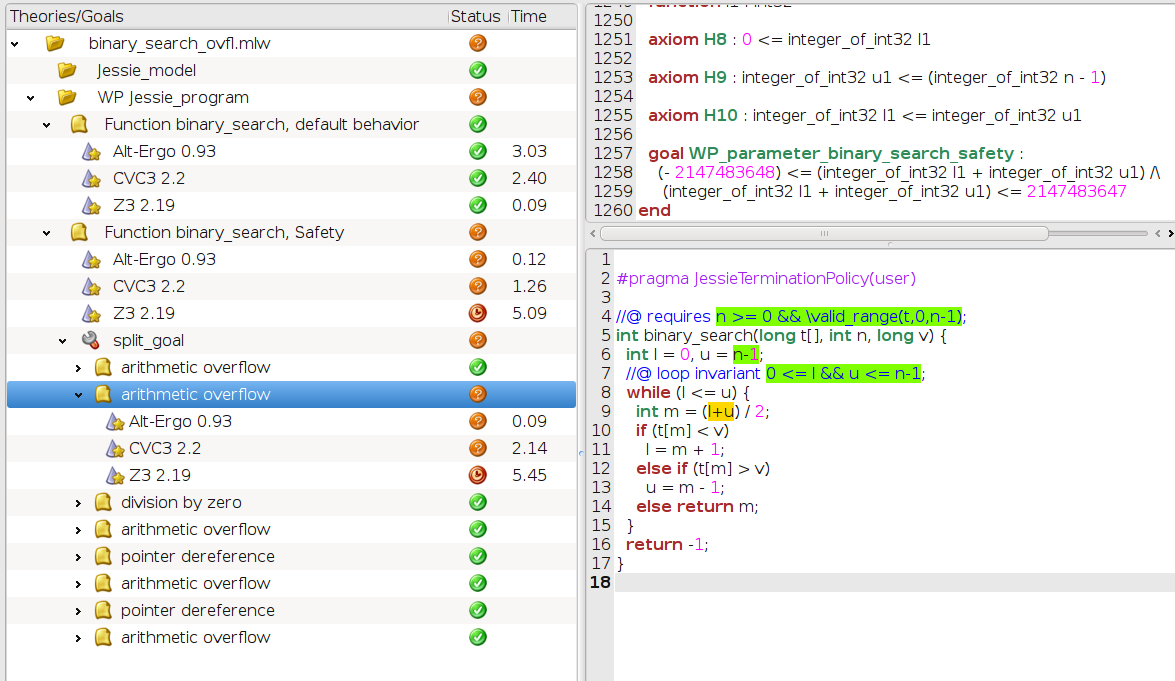
\includegraphics[width=\linewidth]{jessie/binary_search_ovfl.png}
  \caption{Memory safety + integer overflow safety}
  \label{fig:ovfl}
  \hrulefill
\end{figure}

The result can be seen in Figure~\ref{fig:ovfl}. There are more
subgoals to Safety VC, to check that integer operations return a
result within bounds, only one of which is not proved. With this
exception, the results are nearly the same as with exact integers

The only unproved VC expresses that \verb|l+u| does not overflow. 
Nothing prevents this from happening with our current
precondition for function \verb|binary_search|~\cite{Tuch_KN_07}. There are two
possibilities here. The easiest is to strengthen the precondition
by requiring that \verb|n| is no more than half the maximal signed
integer \verb|INT_MAX|. The best way is to change the source of
\verb|binary_search| to prevent overflows even in presence of large
integers. It consists in changing the buggy line

\begin{verbatim}
    int m = (l + u) / 2;
\end{verbatim}

into

\begin{verbatim}
    int m = l + (u - l) / 2;
\end{verbatim}

This is our choice here. All VCs
are now proved automatically.

\section{Checking Termination}

The last kind of safety property we want is termination. To check it,
we first remove the pragma \texttt{JessieTerminationPolicy}. If we run
the VC generation again, we get an additional VC that requires to prove
the property $0 > 0$. This VC is false, so our first step should be
to help Jessie generate a more provable VC.
The VC $0 > 0$ is generated because we did not provide any
\emph{loop variant} for the \texttt{while} loop. A loop variant is a
quantity which must decrease strictly at each loop iteration, while
provably remaining non-negative for as long as the loop runs. 
In this example, a proper variant is $u-l$. 
So our annotated program now looks as follows:

\input{texpp/binary_search_term.cpp}

The additional VC is now proved.

Termination of recursive functions can be dealt with similarly by
adding a \texttt{decreases} clause to the function's contract. 
It is also possible to prove termination by using variants over 
any datatype $d$ equipped with a well-founded relation. 
See the ACSL documentation for details.


% \section{Combining with Value analysis plug-in}

% TODO

\chapter{Functional Verification}


\section{Behaviors}

\subsection{Simple functional property}

Now that the safety of function \verb|binary_search| has been established, one
can attempt the verification of functional properties, like the
input-output behavior of function \verb|binary_search|. At the
simplest, one can add a postcondition that \verb|binary_search| should
respect upon returning to its caller. Here, we add bounds on the value
returned by \verb|binary_search|. To prove this postcondition,
strengthening the loop invariant is necessary.

\input{texpp/binary_search_post.cpp}

All VCs are proved automatically here.

\subsection{More advanced functional properties}

\begin{figure}[t]
  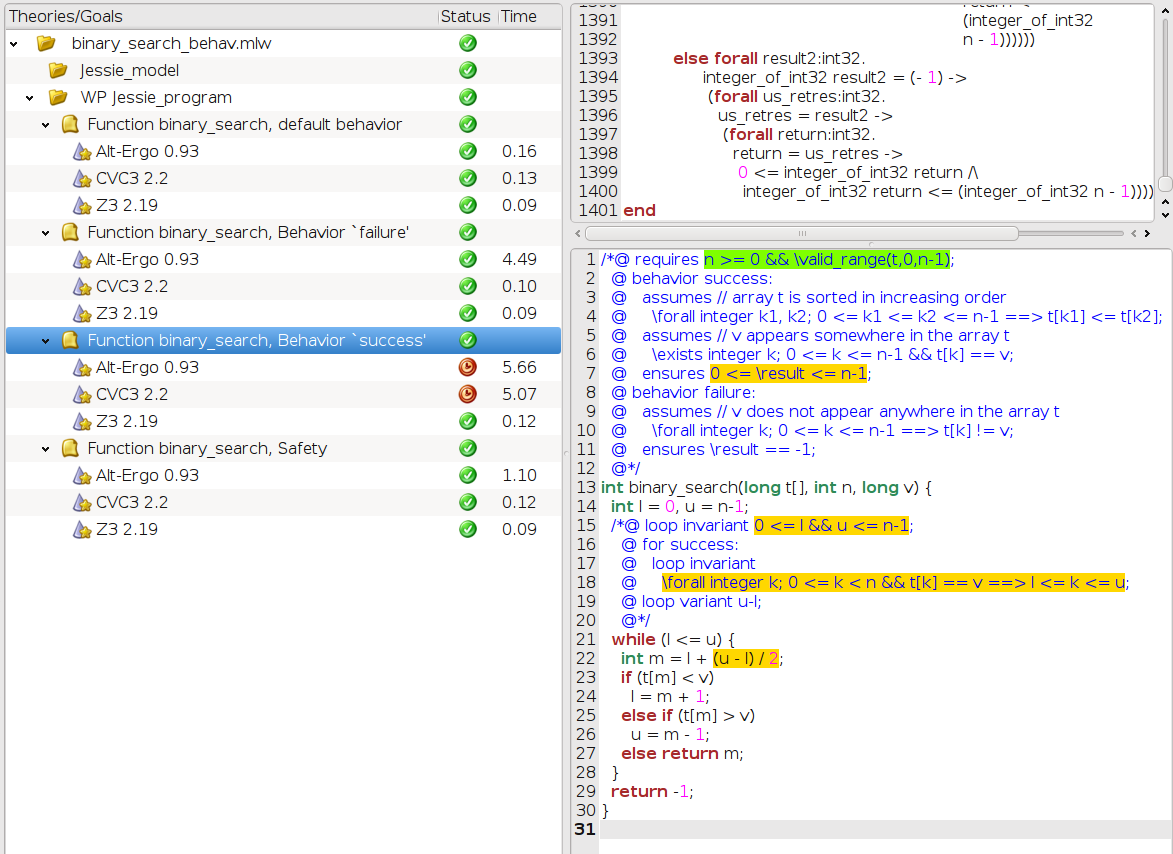
\includegraphics[width=\linewidth]{jessie/binary_search_behav.png}
  \caption{Postconditions in behaviors}
  \label{fig:behav}
  \hrulefill
\end{figure}

One can be more precise and separate the postcondition according to
different behaviors. The \emph{assumes} clause of a behavior gives
precisely the context in which a behavior applies. Here, we state that
function \verb|binary_search| has two modes: a success mode and a
failure mode. This directly relies on array \verb|t| to be sorted,
thus we add this as a general requirement. The success mode states
that whenever the calling context is such that value \verb|v| is in
the range of \verb|t| searched, then the value returned is a valid
index. The failure mode states that whenever the calling context is
such that value \verb|v| is not in the range of \verb|t| searched,
then function \verb|binary_search| returns \verb|-1|.  Again, it is
necessary to strengthen the loop invariant to prove the VC generated.

\input{texpp/binary_search_behav.cpp}

Figure~\ref{fig:behav} summarizes the results obtained in that case,
for each behavior.

\section{Advanced Algebraic Modeling}

The following example introduces use of algebraic specification. The
goal is the verify a simple sorting algorithm (by extraction of the
minimum).

The first step is to introduce logical predicates to define the
meanings for an array to be sorted in increasing order, to be a
permutation of another. This is done as follows, in a separate file
say \texttt{sorting.h}

\input{texpp/sorting.hpp}

The code is then annotated using these predicates as follows

\input{texpp/selection_sort.cpp}

Each VC is proved by at least by Z3. The behavior ``sorted'' is the
most diificult one. Indeed, if you split this one into subgolas, then
all subgoals are proved by Alt-Ergo too.

\chapter{Separation of Memory Regions}

By default, the Jessie plug-in assumes different pointers point into
different memory \textit{regions}.  E.g., the following postcondition
can be proved on function \verb|max|, because parameters \verb|r|,
\verb|i| and \verb|j| are assumed to point into different regions.

\input{texpp/max_ptr_sep.cpp}

To change this default behavior, add the following line at the top of the file:
\begin{verbatim}
# pragma SeparationPolicy(none)
\end{verbatim}

In this setting, the postcondition cannot be proved anymore.
Now, function \verb|max| should only be called in a context where
parameters \verb|r|, \verb|i| and \verb|j| indeed point into
different regions, like the following:

\input{texpp/max_sep_ctxt.cpp}

In this context, all VCs are proved.

In fact, regions that are only read, like the regions pointed to by
\verb|i| and \verb|j|, need not be disjoint. Since nothing is written
in these regions, it is still correct to prove their contract in a
context where they are assumed disjoint, whereas they may not be
disjoint in reality. It is the case in the following context:

\input{texpp/max_sep_ctxt2.cpp}

In this context too, all VCs are proved.

Finally, let's consider the following case of a context in which a
region that is read and a function that is written are not disjoint:

\input{texpp/max_sep_ctxt3.cpp}

The proof that regions are indeed disjoint boils down to proving that
set of pointers \verb|{&a}| and \verb|{&a}| are disjoint (because
function \verb|max| only writes and reads \verb|*r| and \verb|*i|),
which is obviously false.


\chapter{Reference Manual}

\section{General usage}
\label{sec:general}

The Jessie plug-in is activated by passing option
\verb|-jessie| to \verb|frama-c|. Running the Jessie plug-in
on a file f.jc produces the following files:

\begin{itemize}
\item f.jessie: sub-directory where every generated files go
\item f.jessie/f.jc: translation of source file into intermediate Jessie language
\item f.jessie/f.cloc: trace file for source locations
\end{itemize}

The plug-in will then automatically call the Jessie tool of the Why
platform to analyze the generated file f.jc above. By default, VCs are
generated using Why3 VC generator and displayed in the Why3IDE
interface. Using \verb|-jessie-atp=gui| option will use the Why2 VC
generator and display in the Why GUI interface, as it was the default
in version 2.29 and before (deprecated).

The \verb|-jessie-atp=<p>| option allows to run VCs in batch, using
the given theorem prover \texttt{<p>}. It uses the Why2 VC
generator only, and is thus deprecated. Running prover in batch mode
after using the Why3 VC generator can be done using Why3 tools
\verb|why3bench| or \verb|why3replayer|, see Why3 manual for details.


\section{Unsupported features}

\subsection{Unsupported C features}

\begin{description}
\item[Arbitrary gotos] ~\\
  only forward gotos, not jumping into nested
  blocks, are allowed. There is no plan to support arbitrary gotos in
  a near future.
\item[Function pointers] ~\\
  There is no plan to support them in a near
  future. In some cases, Frama-C's specialization plug-in can be used to
  remove function pointers.
\item[Arbitrary cast] ~\\
  \begin{itemize}
  \item from integers to pointers, from pointer to integers: no support
  \item between pointers: experimental support, only for casts in code, not logic
  \end{itemize}
  Note: casts between integer types are supported
\item[Union types] ~\\
  experimental support, both in code and annotations
\item[Variadic C functions] ~\\
  unsupported

\item[\texttt{volatile} declaration modifier]~\\
  not supported
\item[\texttt{const} declaration modifier]~\\
  accepted but not taken into account, that is treated as non-const.

\end{description}


\subsection{partially supported ACSL features}

\begin{description}
\item[Inductive predicates] ~\\
  supported, but must follow the positive
  Horn clauses style presented in the ACSL documentation.
\item[Axiomatic declarations] ~\\
  supported (experimental)
\end{description}

\subsection{Unsupported ACSL features}

\begin{description}
\item[Logic language] ~\\
  \begin{itemize}
  \item direct equality on structures is not supported. Equality of
    each field should be used instead (e.g. by introducing an adequate
    predicate). Similarly, direct equality of arrays is not supported,
    and equality of each cells should be used instead.
  \item array and structure field functional modifiers are not supported
  \item higher-order constructs \verb|\lambda|, \verb|\sum|,
    \verb|\prod|, etc. are not supported
  \end{itemize}
\item[Logic specifications] ~\\
  \begin{itemize}
  \item model variables and fields
  \item global invariants and type invariants
  \item \verb|volatile| declarations
  \item \verb|\initialized| and \verb|\specified| predicates
  \end{itemize}
\item[Contract clauses] ~\\
  \begin{itemize}
  \item \texttt{terminates} clause
  \item abrupt termination clauses
  \item general code invariants (only loop invariants are supported)
  \end{itemize}
\item[Ghost code] ~\\
  \begin{itemize}
  \item it is not checked whether ghost code does not interfere with
    program code.
  \item ghost structure fields are not supported
  \end{itemize}

\end{description}

\section{Command-line options}

\begin{description}
\item[-jessie]
  activates the plug-in, to perform C to Jessie translation

\item[-jessie-project-name=<s>]
  specify project name for Jessie analysis

\item[-jessie-atp=<s>] See Section~\ref{sec:general}. Deprecated.
% do not launch the GUI but run specified
%   automated theorem prover in batch (among \verb|alt-ergo|,
%   \verb|cvc3|, \verb|simplify|, \verb|yices|, \verb|z3|), or just
%   generate the verification conditions (\verb|goals|)

\item[-jessie-cpu-limit=<i>] set the time limit in sec. for proving
  each VC. Only works when \verb|-jessie-atp| is set. Deprecated.

\item[-jessie-behavior=<s>] restrict verification to the given
  behavior (\texttt{safety}, \texttt{default} or a user-defined
  behavior)

\item[-jessie-std-stubs]
  (obsolete) use annotated standard headers

\item[-jessie-hint-level=<i>]
  level of hints, i.e. assertions to help the
  proof (e.g. for string usage)

\item[-jessie-infer-annot=<s>]
  infer function annotations (inv, pre, spre, wpre)

\item[-jessie-abstract-domain=<s>]
  use specified abstract domain (box, oct or poly)

\item[-jessie-jc-opt=<s>] give an option to
  the jessie tool (e.g., -trust-ai)

\item[-jessie-why-opt=<s>]
  give an option to Why (e.g., -fast-wp)
\end{description}

\section{Pragmas}

\begin{description}
\item[Integer model]~\\

  \texttt{\# pragma JessieIntegerModel}(value)

  Possible values: \texttt{math}, \texttt{defensive}, \texttt{modulo}.

  Default value: \texttt{defensive}
  \begin{itemize}
  \item \texttt{math}: all int types are modeled by mathematical,
    unbounded integers ;
  \item \texttt{defensive}: int types are modeled by integers with
    appropriate bounds, and for each arithmetic operations, it is
    mandatory to show that no overflow occur ;
  \item \texttt{modulo}: models exactly machine integer arithmetics,
    allowing overflow, that is results must be taken modulo $2^n$ for
    the appropriate $n$ for each type.
  \end{itemize}

\item[Floating point model] ~\\

  \texttt{\# pragma JessieFloatModel}(value)

  Possible values: \texttt{math}, \texttt{defensive}, \texttt{full},
  \texttt{multirounding}.

  Default value: \texttt{defensive}.

  \begin{itemize}
  \item \texttt{math}: all float types are modeled by
    mathematical unbounded real numbers
  \item \texttt{defensive}: float types are modeled by real numbers
    with appropriate bounds and roundings, and for each floating-point
    arithmetic operations, it is mandatory to show that no overflow
    occur. This model follows the IEEE-754 standard, under its
    \emph{strict} form, as explained in~\cite{ayad09,ayad10ijcar}.
  \item \texttt{full}: models the full IEEE-754 standard, including
    infinite values and NaNs. This model is the \emph{full} model
    discussed in~\cite{ayad09,ayad10ijcar}.
  \item \texttt{multirounding}: models floating-point arithmetics so
    as to support combinations of compilerd and architectures that do
    not strictly follows IEEE-754 standard (e.g. double roundings,
    80-bits extended formats, compilation usinf fused-multiply-add
    instructions). This is based on paper~\cite{boldo09misc,boldo10-nfm}.

  \end{itemize}

\item[Floating point rounding mode] ~\\

  \texttt{\# pragma JessieFloatRoundingMode}(value)

  Possible values: \texttt{nearesteven}, \texttt{down}, \texttt{up},
  \texttt{tozero}, \texttt{nearestaway}.

  Default value: \texttt{nearesteven}.


\item[Separation policy]~\\

  \texttt{\# pragma SeparationPolicy}(value)

  Possible values: \texttt{none}, \texttt{regions}

\item[Invariant policy]~\\

  \texttt{\# pragma InvariantPolicy}(value)

  Possible values: \texttt{none}, \texttt{arguments}, \texttt{ownership}

\item[Termination policy]~\\

  \texttt{\# pragma JessieTerminationPolicy}(value)

  Possible values: \texttt{always}, \texttt{never}, \texttt{user}

  Default: \texttt{always}

  \begin{itemize}
  \item \texttt{always} means that every loop and every recursive
    function should be proved terminating. If they are not annotated
    by variants, then an unprovable VC ($0<0$) is generated.

  \item \texttt{user} means that VCs for termination are generated for
    each case where a loop or function variant is given. Otherwise no
    VC is generated.

  \item \texttt{never} means no VC for termination are ever generated,
    even for annotated loop or recursive function.

  \end{itemize}

\end{description}

% \chapter{Further reading}

% \begin{itemize}
% \item ACSL By Example: Towards a Verified C Standard
%     Library \url{http://www.first.fraunhofer.de/device_soft_en}.
% \item TODO: Moy thesis, Lecture notes of types summer school, voos
%   winter school.
% \end{itemize}

\section{Troubleshooting}

Here is a set of common error messages and possible fix or workaround.
\begin{description}

\item [unsupported "cannot handle this lvalue"]
  this message may appear in the following situations:
  \begin{itemize}
  \item use an array as a parameter of a logic function. You should use
    a pointer instead.
  \end{itemize}

\item[unsupported "this kind of memory access is not currently supported"]
    this message may appear in the following situations:
  \begin{itemize}
  \item equality on structures in the logic. The workaround is to
    check equality field by field. Tip: define field-by-field equality as a
    logic predicate.
  \end{itemize}

\item[unsupported "Jessie plugin does not support struct or union as
  parameter to logic functions."]  This
  is already quite explicit: jessie does not support structures or
  unions as a parameter of logic functions or predicates. You can
  circumvent this limitation by using an indirection via a pointer.

\item[unsupported "cannot take address of a function"] The jessie
  plugin does not support functions as parameters to other
  functions. There is no simple workaround. One thing you can try is
  to remove the function parameter and use a fixed abstract function
  (i.e. with a contract but no body), and then prove that all the
  functions that might be passed as parameters respect this contract.

\item[unsupported "Type builtin\_va\_list not allowed"] Jessie does not
  handle varyadic functions. The same trick as above could be
  attempted.

\item[unsupported "Casting from type <..> to type <..> not allowed"]
  Jessie does not support this cast, typically between pointer and
  integer. There is no simple workaround. One way of proving such kind
  of code is to replace the casts by an abstract function, whose
  post-condition explicitly explains how the conversion is made.

\item[failure: cannot interpreted this lvalue]
  This may happen if
  \begin{itemize}
  \item using a structure in an assigns clause. You need to expand ans
    say which field are assigned.
  \end{itemize}

\end{description}


\bibliographystyle{plain}
\bibliography{biblio}

\end{document}

\documentclass[a4paper]{report}
\usepackage{hevea}

\usepackage{hyperref}

\setlength{\textheight}{240mm}
\setlength{\topmargin}{-10mm}
\setlength{\textwidth}{160mm}
\setlength{\oddsidemargin}{0mm}
\setlength{\evensidemargin}{0mm}
\newcommand{\version}{1.4}

%BEGIN LATEX
\renewcommand{\textfraction}{0.01}
\renewcommand{\topfraction}{0.99}
\renewcommand{\bottomfraction}{0.99}
%END LATEX

\usepackage[T1]{fontenc}
\usepackage{times}
%HEVEA \newcommand{\includegraphics}[2][2]{\imgsrc{#2}}
%HEVEA \newcommand{\hrulefill}{\relax}
%HEVEA \newcommand{\negtenthspace}{\relax}
%BEGIN LATEX
\usepackage{graphicx}
\newcommand{\negtenthspace}{\hspace*{-0.1\linewidth}}
%END LATEX

\newcommand{\Eg}{\mbox{\it E.g.}, }
%OLDHEVEA \newcommand{\land}{\wedge}
%OLDHEVEA \newcommand{\lor}{\vee}

\usepackage{xcolor}
\definecolor{darkgreen}{rgb}{0, 0.5, 0}

\ifhevea%
\makeatletter%
\renewenvironment{document}{%
\@end{document}%
\@atbegindocument%
\@restartoutput\unskip%
\@print{<#def title>Jessie Plug-in Tutorial</#def>
<#def meta><meta name="GENERATOR" content="hevea }%
\@getprint{\usebox{\@heveaversion}}\@print{"></#def>
<#head>
}%
\usebox{\@toplinks}\usebox{\@linkstext}%
\cutdef*[\thecuttingdepth]{\cuttingunit}%
\renewcommand{\addstyle}[1]{\hva@warn{\addstyle{} must be used in document preamble}}%
\@open@par%Open first paragraph
}{%
\@clearstyle\@footnoteflush{\@footnotelevel}\cutend*\title@flush@hook%
\@atenddocument%
\@final@footer%
\@clearstyle%
\@print{<#foot>}%
\@raise@enddocument}%
\makeatother%
\fi

\begin{document}

\ifhevea%
This document is also available in
\ahref{jessie/jessie-tutorial.pdf}{pdf format}.
\else
\sloppy
\hbadness=10000
\begin{titlepage}
\includegraphics[height=14mm]{inriasaclaylogo.png}
\vfill
\begin{center} \Large
{\Huge\bfseries    Jessie Plug-In Tutorial}

\Large Frama-C version: \emph{Nitrogen}

Jessie plug-in version: 2.30

\vfill

\large  Claude March\'e$^{1,3}$, Yannick Moy$^{2,3}$, 

\vfill

\today
\end{center}
\vfill

\vfill
\begin{flushleft}
$^1$ INRIA Saclay - \^Ile-de-France, ProVal, Orsay, F-91893 \\
$^2$ France T\'el\'ecom, Lannion, F-22307 \\
$^3$ LRI, Univ Paris-Sud, CNRS, Orsay, F-91405
\end{flushleft}
  \textcopyright 2009-2014 CNRS/INRIA/Univ Paris-Sud

  This work was supported by the `CAT' ANR project
  (ANR-05-RNTL-0030x), the ANRT CIFRE contract 2005/973, and the `U3CAT'
  ANR project.
\end{titlepage}
\fi




\cleardoublepage
\label{chap:contents}
\tableofcontents

%%% Local Variables:
%%% mode: latex
%%% TeX-PDF-mode: t
%%% TeX-master: t
%%% End:




